\documentclass[runningheads]{llncs}
\usepackage[T1]{fontenc}
\usepackage{tikz}
\usetikzlibrary{positioning, shapes.misc}

\begin{document}

\begin{figure}[t]
    \centering
    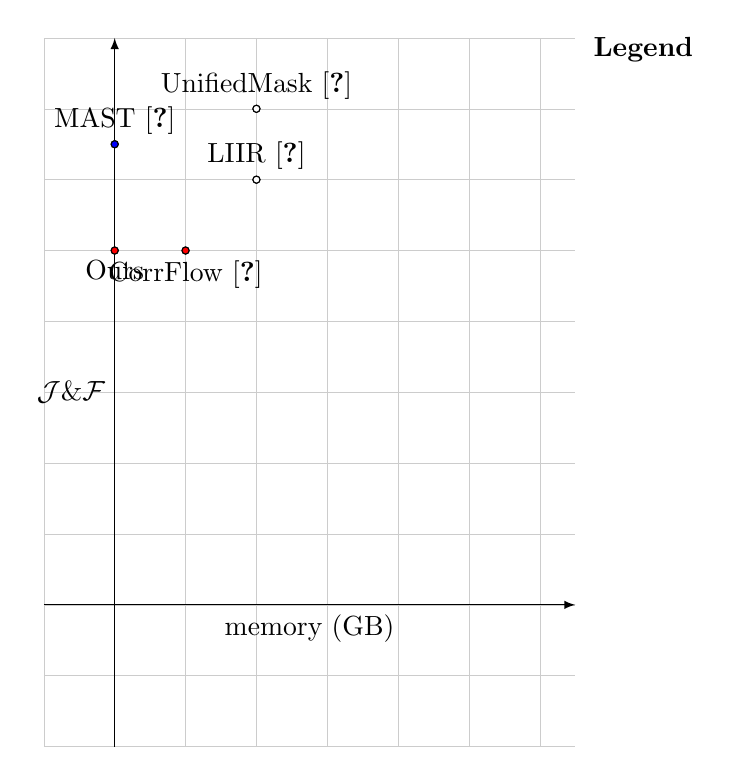
\begin{tikzpicture}[scale=0.9]
        % Grid
        \draw[help lines, color=gray!40] (-1,-2) grid (6.5,8);
        % Axis
        \draw[-latex] (-1,0) -- node[below] {memory (GB)} (6.5,0);
        \draw[-latex] (0,-2) -- node[left] {$\mathcal{J}\&\mathcal{F}$} (0,8);
        % Data points
        \draw[fill=blue] (0,6.5) circle (0.05) node[anchor=south] {MAST~\cite{mastr19}};
        \draw[fill=red] (0,5) circle (0.05) node[anchor=north] {Ours};
        \draw[fill=red] (1,5) circle (0.05) node[anchor=north] {CorrFlow~\cite{corrflow21}};
        \draw[fill=white] (2,6) circle (0.05) node[anchor=south] {LIIR~\cite{liir21}};
        \draw[fill=white] (2,7) circle (0.05) node[anchor=south] {UnifiedMask~\cite{unifiedmask22}};
        % Legend
        \draw[fill=blue] (0,6.5) circle (0.05);
        \draw[fill=red] (0,5) circle (0.05);
        \draw[fill=red] (1,5) circle (0.05);
        \draw[fill=white] (2,6) circle (0.05);
        \draw[fill=white] (2,7) circle (0.05);
        \node [anchor=west,xshift=1mm,yshift=-1.5mm] at (current bounding box.north east) {\textbf{Legend}};
        \end{tikzpicture}
    \caption{Comparison of self-supervised/unsupervised VOS methods in terms of segmentation accuracy ($\mathcal{J}\&\mathcal{F}$) and memory footprint on DAVIS-17 Val dataset.}
    \label{fig:supervos}
\end{figure}

\end{document}